% this document structures the dissertation and should have minimal content

% TODO List;
%   * Fix acronyms not capitalised at beginning of sentence
%   * Fix figure positioning
%   * Todo (indicated with phrase 'Zambingo')

% this document structures the dissertation and should have minimal content

% TODO List;
%   * Fix acronyms not capitalised at beginning of sentence
%   * Fix figure positioning
%   * Todo (indicated with phrase 'Zambingo')

\documentclass[12pt]{uwthesis17}

\usepackage{hon_dissert} % contains entire preamble

% despite not using any chron timelines, this package is now a dependency... - don't remove
\usepackage{chronology} % custom sty file - switched to ggplot (redundant)

\title{Flip Probability as a Loss Function in Convolutional Neural Networks for Image Classification}
\author{Matthew Keith Skiffington} 
\begin{document}
\pagenumbering{roman}
\maketitle
\setcounter{page}{2}

\setlength{\parindent}{0pt} % disable indents

\begin{abstract}

We developed a novel implementation of a \gls{loss} function; the empirical \gls{flipprobability}, derived from the flip probability developed by Durrant \& Kab\'an \cite{durrant2013sharp}. \gls{loss} and tested it in several canonical versions of convolution neural networks to assess whether an increase in training speed or \gls{generalisationperformance} could be achieved. While the \gls{lossfunction} can be used to train networks of a reasonably high accuracy, the performance is generally worse than when standard a standard \gls{lossfunction} and architecture is used. 

\end{abstract}
\begin{acknowledgements}

\bigskip

\begin{spacing}{2}

% ZAMINGO - is it 'was pivotal' or 'were pivotal'?
% removed - I think it overstates the results
% Check whether '.' after Dr
I would like to thank Dr Robert Durrant for his patience, wisdom and understanding in helping produce this dissertation.
\bigskip

I am grateful for the support and kindness of my partner, Renata Sawyer.
\bigskip

\end{spacing}

\end{acknowledgements}
\tableofcontents
\listoffigures
\listoftables

% haven't figured this one out yet in a way that doesn't conflict with existing packages
% \listofmyequations


\newpage
\pagenumbering{arabic}
\setcounter{page}{1}
% these glossary entries are defined off the 'top of my head' i.e. off my current understanding. Where a source has been used for the def I have cited it.

\newglossaryentry{attributes}
{
    name=attributes,
    description={In a machine learning context, these are the variables or columns of the data (e.g. the pixel grayscale intensity values used during image classification, or the weight of an individual used in predicting diabetes risk)}
}

\newglossaryentry{activationfunction}
{
    name=activation function,
    description={A non-linear mathematical function, such as the rectified linear unit the weighted sum of a neuron is put through in order introduce a non-linearity in the network to improve learning}
}

\newglossaryentry{backpropagation}
{
    name=back propagation,
    description={The process of calculating the gradients based on the size of the loss with respect to all of the parameters in the network, using the chain rule, and updating the parameters in direction that minimises the loss (using some optimisation method)}
}

\newglossaryentry{classlabel}
{
    name=attributes,
    description={The attribute that indicates the true class of the observation or example (e.g. "cat" or "dog" for pet images)}
}

\newglossaryentry{costfunction}
{
    name={cost function},
    description={A synonym for a loss function \cite[p.~80]{good_fellow_2016}.}
}

\newglossaryentry{dataaugmentation} % TODO - improve this glossary entry
{
    name=data augmentation,
    description={The practice of applying a transformation to the raw data and training the given algorithm on the transformed data (as well as, in certain cases, the transformed data). Examples include generating extra examples using generative adversarial networks, rotating images and normalising input data}
}

\newglossaryentry{decisionboundary}
{
    name=decision boundary,
    description={The geometric boundary in the space of data where the algorithm will go from predicting one class (e.g. setosa), to another class (e.g. versicolor)}
}

\newglossaryentry{epoch}
{
    name=epoch,
    description={A full forward and backwards pass over the network}
}

\newglossaryentry{features}
{
    name=features,
    description={Attributes}
}

\newglossaryentry{feedforward}
{
    name=feed forward,
    description={A simple type of neural network where each neuron in the previous layer is connected to every neuron in the next layer} 
}

\newglossaryentry{flipprobability}
{
    name=flip probability,
    description={The probability that the classification of a label will flip given a classifier if the data is randomly projected down to a lower dimensional subspace}
}

\newglossaryentry{forwardpropagation}
{
    name=forward propagation,
    description={The process of running the input data through the layers of network to produce some output}
}

\newglossaryentry{generalisationperformance}
{
    name=flip probability,
    description={How well the classifier performs on new, unseen data not used in either the testing in training data sets}
}

\newglossaryentry{hyperparameter}
{
    name=hyperparameter,
    description={A parameter that governs the training of the model,such as the batch size used in \gls{sgd}} 
}

\newglossaryentry{hyperplane}
{
    name=hyperplane,
    description={A geometric term. A plane is the layman's sense is a 2D surface in 3D space. A hyperplane is the flat equivalent (n-1)-d surface, in an n-d space (this can include the straight-forward 3d context - hence a sheet of paper can be described as a 'hyperplane', if we were to pretend it had zero thickness)}
}

\newglossaryentry{imagerecognition}
{
    name=image recognition,
    description={A synonym for image classification}
}

\newglossaryentry{indicatorfunction}
{
    name=indicator function,
    description={A function that takes the value one if its condition is true or zero if its condition is false}
}

% TODO

\newglossaryentry{layer}
{
    name=layer,
    description={A set of neurons in a neural network that receive data from either the input (data) layer or the output of the previous layer of neurons. Mathematically this can be thought of as a matrix of weights, with a bias column appended (if a bias term is included) } 
}

\newglossaryentry{linearclassifier}
{
    name=linear classifier,
    description={A classifier which uses a linear combination of the features to classifier the data and so forms a straight (in 2D) or flat (or 3D) decision boundary}
}

\newglossaryentry{linearlyseparable}
{
    name=linearly separable,
    description={Able to be separated by a linear classifier}
}

\newglossaryentry{lossfunction}
{
    name=loss function,
    description={A function that calculates the loss. We usually wish to minimise (or in some cases, maximise) the result of this function as part of some optimisation procedure}
}

\newglossaryentry{loss}
{
    name=loss,
    description={A statistical measure of the distance between the predicted result and the actual result, used in the training of learning algorithms}
}

\newglossaryentry{neuralnetwork}
{
    name={NN},
    description={A Neural Network (NN) is a machine learning algorithm that comprises of a series of layers each with a given number of neurons (which act as a weighted sum of the inputs) with trainable parameters including weights and biases where each neuron typically undergoes a non-linear transformation in the form of an activation function to ultimately produce a prediction of class or target value based on the input data}
}

\newglossaryentry{neuron}
{
    name=layer,
    description={ In a neural network context, a neuron is a single 'unit' that applies a function. Mathematically, this can be thought of as a single column in a the weights matrix, with a length that matches the dimensionality for the input data (if the neuron is situated in the input layer).  } 
}

\newglossaryentry{objectivefunction}
{
    name={objective function},
    description={A synonym (generally) for a loss function \cite[p.~80]{good_fellow_2016}}
}

\newglossaryentry{parameterspace}
{
    name={parameter space},
    description={The parameter space of the model or algorithm is the n-dimensional space in which a single point would represent a single combination of the parameters.}
}

\newglossaryentry{representationlearning}
{
    name=representation learning,
    description={A method of initially learning a simpler transformed representation from the raw data that allows for superior classification by a (usually linear) classifier}
}

\newglossaryentry{resnet}
{
    name=residual network,
    description={A type of deep neural network that uses residual connections (which use the identity function) between layers to allow improved gradient flow and gain increased accuracy from additional layers}
}

\newglossaryentry{semanticsegmentation}
{
    name=semantic segmentation,
    description={The task of breaking down any image (input data) into labelled discrete sections that have some semantic meaning. For example, breaking down 'The Persistence of Memory' by Dali into 'watch', 'sky', 'ground', 'water', etc.}
}

\newglossaryentry{softmax}
{
    name=soft max,
    description={A loss function used in classification problems which } % todo 
}

\newglossaryentry{supervisedlearning}
{
    name=supervised learning,
    description={Any learning that uses the class label or true target value (e.g. linear regression)}
}

\newglossaryentry{unsupervisedlearning}
{
    name=unsupervised learning,
    description={Any learning that does not use the class label or true target value (e.g. clustering)}
}

\newacronym{ai}{AI}{Artificial Intelligence}
\newacronym{apm}{APM}{Actions Per Minute}
\newacronym{ann}{ANN}{Artificial Neural Network} 
\newacronym{adam}{ADAM}{Adaptive Moment Estimation} 
\newacronym{aws}{AWS}{Amazon Web Services}
\newacronym{cifar}{CIFAR}{Canadian Institute for Advanced Research}
\newacronym{cnn}{CNN}{Convolutional Neural Network}
\newacronym{cpu}{CPU}{Central Processing Unit}
\newacronym{cv}{CV}{Cross Validation}
\newacronym{dl}{DL}{Deep Learning}
\newacronym{dnn}{DNN}{Deep Neural Network}
\newacronym{dcnn}{DCNN}{Deep Convolutional Neural Network}
\newacronym{drl}{DRL}{Deep Reinforcement Learning}
\newacronym{ffnn}{FFNN}{Feedforward Neural Network}
\newacronym{flda}{FLDA}{Fisher's Linear Discriminant Analysis}
\newacronym{fp}{FP}{Flip probability} 
\newacronym{gan}{GAN}{Generative Adversarial Networks} 
\newacronym{gb}{GB}{Gigabyte}
\newacronym{gcp}{GCP}{Google Cloud Platform}
\newacronym{gd}{GD}{Gradient Descent}
\newacronym{gpu}{GPU}{Graphics Processing Unit} 
\newacronym{ilsvrc}{ILSVRC}{ImageNet Large Scale Visual Recognition Challenge}
\newacronym{jll}{JLL}{Johnson-Linden Straus Lemma} 
\newacronym{kl}{KL}{Kullback–Leibler} 
\newacronym{lln}{LNN}{Law of Large Numbers}
\newacronym{ltsm}{LTSM}{Long-Term Short-Term Memory}
\newacronym{ml}{ML}{Machine Learning}
\newacronym{mlp}{MLP}{Multi-layer Perceptron}
\newacronym{mnist}{MNIST}{Modified National Institute of Standards and Technology} 
\newacronym{mse}{MSE}{Mean Squared Error} 
\newacronym{nin}{NIN}{Network-in-Network}

\newglossaryentry{nn}{type=\acronymtype, 
name={NN}, 
description={Neural Network}, 
first={Neural Network (NN)\glsadd{neuralnetwork}},
see=[Glossary:]{neuralnetwork}}

\newacronym{ram}{RAM}{Random Access Memory}
\newacronym{relu}{ReLu}{Rectified Linear Unit}
\newacronym{r-cnn}{RNN}{Region-Convolutional Neural Network}
\newacronym{rnn}{RNN}{Recurrent Neural Network}
\newacronym{rp}{RP}{Random Projection}
\newacronym{sgd}{SGD}{Stochastic Gradient Descent}
\newacronym{ssd}{SSD}{Solid State Disk}
\newacronym{svm}{SVM}{Support Vector Machines}
\newacronym{uap}{UAP}{Universal Approximation Theorem}
\newacronym{vae}{VAE}{Variational Auto-Encoder}
\newacronym{vc}{VC}{Vapnis-Chervonenkis}
\newacronym{xor}{XOR}{Exclusive OR}
\newacronym{yolo}{YOLO}{You Only Look Once}
\include{tex/introduction}
\chapter{Literature Review}

% Split into two main sections: fields and techniques; mathematical background

% Lit review structure
% ML intro as subset of AI
% NNs
% Note on AI winter
% SVMs
% DL emerges - note on previous aspersions on this
% Image recognition
% Expansion to other domains and architectures
% Acceleration, hype (media coverage, publicity etc, large industrial use Tesla etc)
% Emphasis on loss functions and explanation
% History of Random Projections
% Narrow down to flip probability specifically
% Mention use in logistic regression and bounds on error for linear classification

\section*{Fields and Techniques}

%\begin{SCfigure}
% ZAMBINGO - if possible, redo figure using ggplot
% ZAMBINGO - spelling mistake - should be 'breadth' not 'breath
\begin{wrapfigure}{r}{0.5\textwidth}
    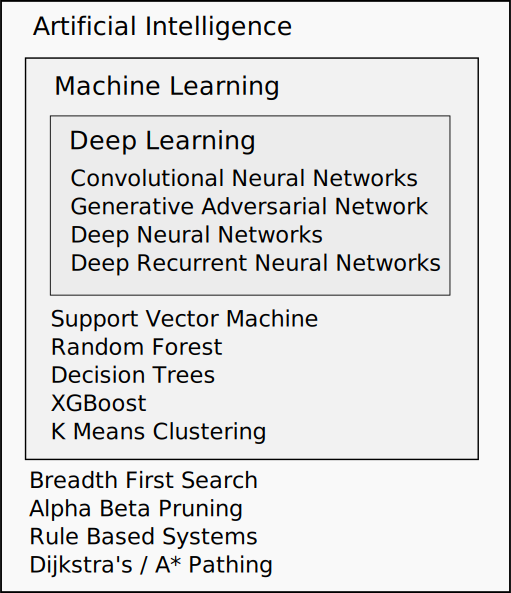
\includegraphics[width=60mm]{figs/ai_ml_dl.png}
    \caption{The fields of \gls{ai}, \gls{ml} and \gls{nn}, with examples of techniques in each.}
    \label{fig:ai_ml_dl} 
\end{wrapfigure}

%\end{SCfigure}

% link between perceptron and logistic regression clarified
% https://stats.stackexchange.com/questions/162257/whats-the-difference-between-logistic-regression-and-perceptron
Figure \ref{fig:ai_ml_dl} shows the relationship between \gls{ai}, \gls{ml} and \gls{dl}. \gls{ai} concerns the broad field of using technology to mimic human behaviour. \gls{ml} additionally involves training algorithms to find rules automatically based on training data, which can involve techniques usually situated within statistics, such as linear or logistic regression. \gls{dl} takes this a step further, concern the use of multi-layered \gls{nn}s trained on a large pool of training data to perform even more complex tasks, such as image segmentation or video captioning. The roots of \gls{ai} goes to the 1940s and 50s, with one particular event, the Dartmouth Summer Research Project, gaining particular retrospective notoriety for proposing to making significant advances in the field in a '2 month, 10 man study'  \cite{dartmouth_summer}. From a statistical perspective, using \gls{nn}s falls within the 'algorithmic modelling' camp, as elaborated by Leo Breiman in \cite{two_cultures}. The emphasis is on predictive accuracy, not finding a data model.

\section{Machine Learning}
% name drop kernel trick

\gls{ml} is an interdisciplinary field at the intersection of mathematics, computer science and statistics and itself is often considered as a sub-field of the broad area of study that is  \gls{ai}. \gls{ml} deals with the challenge of "learning" from data without manual human input. In contrast to many statistical techniques, \gls{ml} is especially suited to scenarios where predictive accuracy is paramount, training examples are both numerous and high dimensional, and inferential understanding is not critical [ZAMBINGO]. \gls{ml} gathered a lot of momentum in the 1990s, with the term 'data mining' often used as a pseudonym. Traditional techniques in the field of \gls{ml} include decision trees,  \gls{svm}s (1992, \cite{svm}, K-means clustering (1962 \cite{k_means}, Naive Bayes and  \gls{flda}.  \bigskip

% probably delete this line 
Examples of classic data sets in \gls{ml} refer to unsupervised classification of data points into flower species, predicting diabetes risk based on a small subset of predictors, predicting whether a mine is present based on hundreds of frequency reflection variable and other challenges \cite{uci_ml_data}. Practical milestones include the use of Yan Le Cun's 'LeNet' architecture in the late 1990s to perform accurate handwriting recognition. 

%At one stage, this algorithm (a \gls{cnn}) was responsible for the majority of automated cheque processing in the United States [ZAMBINGO].  \bigskip

The key idea is that the algorithm automatically finds and determines a set of rules to effectively label the input data based on some learning process that seeks to find the optimal set of model parameters. This avoids, for example, algorithms that are highly task specific (such as searching algorithms or algorithms specifically designed to find the optimal move given a particular rule set). \bigskip

\section{Neural Networks} 

% ZAMBINGO - mention hebbian learning

\gls{nn}s (in this work, networks, \gls{ann}s and 'nets' all refer to \gls{nn}s) started with the linear combiner, which with the addition of extra neurons, become the perceptron \cite{haykin}. With the addition of a \gls{hiddenlayer}, this evolved onto the \gls{mlp}. Later, multi-layer \gls{ffnn}s were used, and the the architecture diversified into the \gls{cnn}s with the use of local receptive fields. A timeline of developments and architectures is present in figures \ref{fig:timeline_new_nn} and \ref{fig:timeline_old_nn}. \bigskip

\begin{figure}
    \centering
    \includegraphics[width=140mm,scale=1.5]{figs/timeline_old_nn.png}
    \caption{A selection of events in early neural network history}
    \label{fig:timeline_old_nn}
\end{figure}

\begin{figure}
    \centering
    \includegraphics[width=140mm,scale=1.5]{figs/timeline_new_nn.png}
    \caption{A selection of events in modern neural network history}
    \label{fig:timeline_new_nn}
\end{figure}

Figures \ref{fig:timeline_old_nn} and \ref{fig:timeline_new_nn} show a small selection of key historic and recent events. 

A \gls{nn} can be interpreted many ways. For example, a common interpretation is that \gls{nn} act as function approximation machines, a view influence by the \gls{uap} theorem for \gls{mlp}s, which states that;

\begin{quote}
    A standard multilayer feedforward network with a locally bounded piecewise continuous activation function can approximate any, continuous function to any degree of accuracy if and only if the network's activation function is not a polynomial.\cite{uap_mlp}
\end{quote}

Another view of \gls{nn}s is as an extremely simply approximation of how the brain works. This has more of a parallel when the heaviside activation function, where, if the input signals of the neuron (the weighted attributes of the \gls{instance}, which can be thought of as analogous to the dendrites of a neuron) surpass a given threshold, the neuron 'fires', sending an output signal down the axon (i.e. returns a one, instead of zero).
\bigskip

At it's simplest a \gls{nn} for binary classification is a single \gls{neuron} comprising of a weighted sum of the input features, the addition of a bias term and the application of an \gls{activationfunction} to provide an output for a given input \gls{instance} $i$. This is summarised in \ref{fig:nn_simple} \footnote{\url{Interactive Example of \gls{nn}s, hosted by TensorFlow.}{https://playground.tensorflow.org/}}.  

\begin{figure}
    \centering
    \includegraphics[width=100mm]{figs/nn_simple.png}
    \caption{The prediction process for a single point of data in a linear combiner.}
    \label{fig:nn_simple}
\end{figure}

\begin{equation}
    y_i = \mathds{1} ((\sum_{j = 1}^m w_j + b_m) > 0)
    \label{eq:nn_simple_pred}
\end{equation}
%\myequations{Prediction for a Linear Combiner}

This network is a binary \gls{linearclassifier}, which has a single \gls{layer} and uses the heaviside \gls{activationfunction} (figure \ref{fig:heavi_function}) and does not use a bias term (would would be added to the weighted sum). The output $y_i$, can be either a one, or a zero. It therefore has a single parameter for each non-class attribute present in the input data, which corresponds to each weight, $w_m$. Choosing an \gls{activationfunction}, $\phi$ when designing networks in modern times often comes down to using the 'tried and true' functions (such as \gls{relu}), or a lot of manual \gls{hyperparameter} tuning.

\begin{wrapfigure}{l}{0.5\textwidth}
    \includegraphics[scale=0.5]{figs/heavi.png}
    \caption{The Heaviside activation function.}
    \label{fig:heavi_function}
\end{wrapfigure}

% spiel about VC dim and linear classifiers using simple logistic regression (and link to NN)
If we use the sigmoid \gls{activationfunction} and incorporate a bias term, we now have what is equivalent to a logistic regression. Hence there is a parallel that can be drawn between a particular configuration of the perceptron, an early technique in \gls{ml} and the traditional statistical logistic regression. By a running a logistic regression with data that has the minimal \gls{vc} dimension (3) for a \gls{linearclassifier}, we can see that the classifier can always 'shatter' (perfectly separate) the data. This is because the \gls{vc} dimension of a linear classifier is $d+1$. However, if we increase the number of points to four (surpassing the \gls{vc} dimension of the classifier), we now find this is not always true (see figure \ref{fig:vc_4}).

\begin{figure}[H]
    \centering
    \includegraphics[width=120mm]{figs/vc_3.png}
    \caption[\Gls{vc} dimension of a linear classifier - the data is shattered.]{In two dimensions, logistic regression (a linear classifier) can perfectly shatter a data set with three points, in all cases. The points have been randomly generated in each plot, a logistic regression fitted to each data set using $x, y$ as covariates.}
    \label{fig:vc_3}
\end{figure}

\begin{figure}[H]
    \centering
    \includegraphics[width=120mm]{figs/vc_4.png}
    \caption[Surpassing the \gls{vc} dimension of a linear classifier - the data is not always shattered.]{\Gls{linearclassifier}s begin to falter once the VC dimension of the classifier is surpassed in the data. The points have been randomly generated in each plot, a logistic regression fitted to each data set using $x, y$ as covariates and the plots are set to automatically highlight instances of imperfect separation of the data.}
    \label{fig:vc_4}
\end{figure}

\begin{wrapfigure}{l}{0.5\textwidth}
    \includegraphics[scale=0.5]{figs/sigmoid.png}
    \caption{The Sigmoid activation function.}
    \label{fig:sigmoid_function}
\end{wrapfigure}

Many \gls{nn} diverge from most statistical techniques in that they do not assume a distribution over the data, rather taking an 'algorithmic' approach to classification and prediction \cite{two_cultures}. They leverage the increased classifier complexity that results from the addition of extra neurons to layers ('going wide') and the addition of \gls{layer}s ('going deep'). This increased complexity comes at the cost of the interpretability, although a variety of techniques are in development to tackle this problem \cite{nn_interpretability}.

\gls{nn}s find their origins in the fields of psychology and electronic engineering, dating back to the days of linear adaptive filters in the \cite{nns_haykins}. This began perceptron model proposed by Rosenblatt \cite{perceptron_paper} as an extension of the McCulloch and Pitts model of the neuron \cite{logical_calculus} \bigskip
% ZAMBINGO - figure idea - branching tree of nn architectures leading to cnns

% REDO DIAGRAM IN GGPLOT2
\begin{figure}
    \centering
    \includegraphics[width=120mm]{figs/xor_problem.png}
    \caption{An illustration of the \gls{xor} problem that a perceptron can not solve. Lines indicate arbitrary examples of \gls{linearclassifier}s.}
    \label{fig:xor_problem}
\end{figure}

The \gls{xor} problem is the simplest possible example of data that is not \gls{linearlyseparable}, and thus not able to be classified using a \gls{linearclassifier}. After the highly influential book,'Perceptrons' proved that the \gls{xor} problem (figure \ref{fig:xor_problem}) could not be solved with a single layer perceptron \cite{perceptrons_book}, interest in \gls{nn}s died off considerably - this is often referred to as the 'AI winter' \cite{ai_winter}. This continues to cause general speculation around whether another such 'winter' will occur \cite{ai_winter_spec}. It has been speculated \cite{perceptron_spec} that this was in part because the idea that \gls{mlp}s could not solve the \gls{xor} problem gained traction, despite the authors acknowledging that it was likely that they could in their book \cite{perceptron_book}. \bigskip

% Can't seem to find a reference for this.
% This culminated in a general decrease in funding and a shift in focus, with leading conferences in the field, such as \gls{nip}s receiving more submissions under the field of data mining than \gls{nn}s, despite being explicitly a conference centered around neural systems

Eventually however, research with layered \gls{nn}s intensified and progress was made, not least in part because of advances in computational power;

\begin{quote}
...the IBM 704 computer that cost \$2 million in 1958, or \$20 million in today’s dollars, could perform 12,000 multiplies per second, which was blazingly fast at the time. The much less expensive Samsung Galaxy S6 phone, which can perform 34 billion operations per second, is more than a million times faster...\cite{unreasonable_dl}
\end{quote}

%todo insert xor figure

\bigskip
Coming out of the AI winter, \gls{nn}s were restricted to four or five layers (never past ten). There was a 'node budget' and a lot of manually configured architecture at the node level. The manually specified architecture of the network was critical to it's success \cite{manual_architecture}, for example in computer vision, where significant amounts of feature engineering was required. 

In 1997, Yan Le Cun developed the first neural network capable of high accuracy digit recognition which outperformed the previously popular \gls{svm} models. \bigskip

% CNN

\section{Deep Learning}

% ZAMBINGO - reference for AI safety would be good here - parameter space, understanding of bounds etc

Highly layered ("deep") \gls{nn}s lie at the heart of \gls{dl} and are in fact all extensions of the \gls{mlp}. The phrase 'deep' has a level of subjectivity around it; clearly, a two \gls{layer} \gls{mlp} is not a \gls{dnn}, but is a 5-layer network 'deep'? The most Other deep algorithms do exist (such as 'deep trees' \cite{deep_forest}) although these are unable to handle complex image classification problems as well as other modern {dnn}s. \gls{dl} is seen as a highly effective strategy in a variety of \gls{ai} applications. As a model, they are far more complex than most statistical models, having millions of parameters \cite{unreasonable_dl}.  \bigskip
% AI winter mention and comeback - LeNet CNNs then cooling SVMs

Major recent events (figure \ref{fig:timeline_new_nn}) include progress made in \gls{drl}, such as teaching a network to effectively play a variety of Atari games without any manual intervention \cite{drl_atari}. Generative networks progressed, with the development of \gls{vae}s, which could generate examples from complex distributions and were then surpassed by the development of \gls{gan}s for the generation of highly realistic examples \cite{gans}. AlphaStar \cite{alphastar} and AlphaGo \cite{alphago} gained a lot of attention \cite{press_alpha_go} \cite{press_alpha_star} for beating top human players in the board game Go and the video game StarCraft II. In the later case, the \gls{ai} was constrained in terms of \gls{apm}, it's view and a realistic observation delay and network latency. Both games are notably complex with the first having an extremely large state space (having a search space of $10^360$ moves, versus $10^{43-123}$ for chess \cite{moves_chess_go}) and the second having a complex continuous real time state space, often requiring  around hundreds \gls{apm} \cite{sc_apm} for top human players. Style\gls{gan}s were notable for effective image style transfer, which was also picked up in the media \cite{press_stylegan} \footnote{An interactive example of this can be found here \url{ZAMBINGO}}.

In terms of \gls{cnn}s, kicked off a flurry in research activity in \gls{dl}, as it was the first \gls{dnn} to win the \gls{ilsvrc}, in 2012 \cite{alex_net} \cite{dl_overview}. \gls{r-cnn}s were notable for classification of regions and \gls{semanticsegmentation} using \gls{cnn}s. 'GoogLeNet' introduce a more parallel architecture with the 'inception' module to achieve higher accuracies \cite{googlenet}. \gls{resnet}s broke new ground with it's extreme depth \cite{resnet} by surpassing 'human level recognition' \cite{resnet_human}. 'SqueezeNets' introduce high performing \gls{cnn}s with far fewer parameters and a smaller memory footprint \cite{squeeze_net}. 
\bigskip

For context \gls{nn}s had now significantly fallen out of favour [ZAMBINGO] and \gls{svm}s were rapidly gaining popularity [ZAMBINGO]. This trend continued until 2012, when the striking performance of AlexNet, a \gls{dcnn}, in the influential annual \gls{ilsvrc} created a lot of interest in \gls{dl}. The remarkable improvements in performance achieved showed the viability of \gls{dl} as an alternative to \gls{svm}s and other techniques, for \gls{imagerecognition}. This demonstration was enabled by several factors contributing to recent rapid developments in \gls{dl}: the availability of \gls{dl} tool-kits, such as Theano and Caffe (2007, 2013 - REF), and Keras, TensorFlow and PyTorch (2015, 2016 ZAMBINGO); advances in computational hardware and accessibility, including powerful purpose-built \gls{gpu}s, access to cloud compute (\gls{aws}, \gls{gcp}, Azure, \gls{tpu}s) and decreasing cost barriers (Google Collab, MatrixDS, note on costs e.g. declining storage costs); and access to large, curated data sets for training (large text corpuses \cite{enron_emails}, image repositories \cite{image_net}) \bigskip

Now, \gls{nn}s can be incredibly deep, from 50-150 layers (depths used with \gls{resnet}s \cite{resnet}) and also quite wide (such as 

% insert summary table of models used in ILSVRC, number of parameters, hardware trained on, architecture, unique features and top 1/3/5 accuracy's

% when to capitalise fields?
While this was a major advancement for \gls{dl} in the problem domain of image classification, progress was being made in other domains such as speech recognition, handwriting recognition, image segmentation, image captioning and generative models \cite{dl_overview}. 
\bigskip % todo - finish list of progress in domains
 
\gls{dl} has evolved as a subset of \gls{ml} methods used for extracting complex semantics from data. \gls{dl} methods have achieved a wide variety of goals that would not otherwise be possible via traditional machine algorithms (such as realistic face generation \footnote{For an excellent example of this, see \url{This Person Does Not Exist}{https://www.thispersondoesnotexist.com/}, for realistic faces generated by StyleGANs})  \bigskip% todo - finish list of goals 

The success of  \gls{dl} has fuelled the development of a plethora of different  \gls{nn} architectures, including \gls{ltsm}s, \gls{rnn}s and \gls{gan}s [ZAMBINGO]. These are now widely used in a variety of applications, such as for text-to-speech, handwriting recognition and art generation (respectively). [ZAMBINGO]  \bigskip 

\section{Convolutional Neural Networks}

\gls{cnn}s were inspired by the 'Neocognitron' of the 1980s \cite{neocognitron_proposal} \cite{neocognitron}. This was notable for having a concept similar to \gls{localreceptivefields} and a strategy similar to the pooling and covolutional that occurs in modern \gls{cnn}s ZAMBINGO. \gls{cnn}s were developed in earnest by in the 1990s, with early uses involving reading cheques \cite{lecun_cheques}. The primary purpose of \gls{cnn}s is \gls{imagerecognition}, although they are also used in time series forecasting (1D \gls{cnn}s) and can be used for 3D recognition, for example using sensors from the Microsoft Kinect (\cite{3d_conv}). \gls{cnn}s hinge on 'local receptive fields' (also known as sparse connectively), which means that each of the input layer neurons have a particular patch of the input data that they connect to. The input data (or function) undergoes a convolution, in that a filter (or kernel) is convolved (slid across) the data. Each successive \gls{neuron} in a given layer \cite[Chapter~5]{good_fellow_2016}

% bit on how convolution works
% bit on pooling (or decimation)
% diagram of dimensionality through network

%removed "generally"

\section{Applications}

Image classification is a subset of the broader area of computer vision, which includes such applications as face , object, feature and landmark detection, feature detection, realistic  generation of class examples and art generation.  
\bigskip
%The field of \gls{dl} is a relatively modern one, and recent developments have been popularised through %making appearances in the media, through the striking use of neural style transfer to make various %surprising images or videos - such as the face of a dollar bill, speak a particular phrase, the Mona %Lisa come to life or even figures like Marilyn Monroe take the stage once more [ZAMBINGO]. 

The underpinnings of the resurgence of \gls{dcnn}s in recent times is linked to the use of \gls{dcnn}s for the ImageNet challenge. Prior to this challenge, \gls{dl} had was not widespread due to several problems; computational resources, sufficient training data, a lack of accessible tool-kits and the "vanishing gradients problem" \cite[Chapter~8]{good_fellow_2016} \cite[p.~93-94]{dl_overview}. Today, there is a wide breadth of techniques in \gls{dl}, from deep \gls{rnn}s for object detection in videos, \gls{gan}s for image and video generation, \gls{dcnn}s for \gls{imagerecognition}, ... 

%Recent major developments include Neural Ordinary Differential Equations

\section{Tools and Hardware}

Given the computational complexity of  \gls{dl} models, the providence of good tools has accelerated the development of algorithms.  Initially, neural networks were implemented i

This later burgeoned with Torch, Caffe, Theano and a variety of disparate frameworks and later evolved into Pytorch, Keras and Tensorflow, which have become the main tools of research and production in the \gls{dl}. All three of these frameworks have implementations in Python as well as a variety of other languages (for example, Keras has recently had a wrapper implemented in R \cite{keras_r}). All modern libraries have \gls{ad} incorporated, meaning it is not neccesary to manually find the derivative of a given function in order to perform back propagation; the partial derivatives of functions and the hence the gradients are automatically calculated.  \bigskip

%  ZAMBIGO
Pytorch, developed by Facebook, is common used due to it's 'Pythonic' implementation and imperative style 


The Keras API is often considered the easiest framework for beginners to pick and use, being positioned at a high level of abstraction relative to Tensorflow and Pytorch. It can interface with Tensorflow, Theano or CNTK  \bigskip

Tensorflow, developed by Google,  \cite{tale_dl}. All three frameworks have the advantage of being completely open source. \bigskip

% this paragraph needs a re-write
It is now possible to use a  \gls{nn} 'off-the-shelf' or pre-trained. This is a common strategy in transfer learning, where \gls{dnn}s trained on large data sets are then trained further on new unseen data (which may, for example, include new classes). To speed up training, only the last layer of these networks may be retrained with the new data, in order to leverage the learning power of the existing network. \bigskip

\section*{Mathematical Background}

% ZAMBINGO - need small section on curse and blessing on dimensionality
% elements of statistical learning
% https://stats.stackexchange.com/questions/15971/what-is-the-curse-of-dimensionality

\gls{nn}s are at heart a mathematical technique and despite the enormous ecosystem of competing tools, technologies and techniques that are continuously developed, an understanding of the mathematical principles involved  is critical to safely understanding their operation, furthering practical implementations from fundamental research and for developing an understanding of the bounds of uncertainty involved in accomplishing different tasks with them, whether it be prediction, classification or a sophisticated multi-task system.

\section{Loss Functions}

% mention NP-hardness loss paper
\gls{lossfunction}s measure how far the prediction a statistical or \gls{ml} algorithm creates from the target. As the algorithm is trained, the loss is minimised. In $\mathds{R}^3$, this can be visualised quite strikingly as trying to find the lowest point in a 'loss landscape' \cite{loss_landscape}. This can be explicitly, such as when using the normal equations to solve exactly for the optimal coefficients, such as in linear regression. Linear regression traditionally uses the  \gls{mse} as a \gls{lossfunction}, more commonly known as the L2 loss in a \gls{ml} context:

\begin{equation}
l_2 := \sum_{i = 1}^N (\hat{y_i} - y_i)^2
% todo - MSE equation 
\end{equation}
%\myequations{Mean Squared Error}

Where;

\begin{itemize}
\item $N$ is the number of examples  
\item $y_i$ is each individual target label  
\item $\hat{y}$ is the predicted class for the individual example 
\end{itemize}

More commonly, some optimisation method is required in order to minimise the \gls{loss}.  At the simplest level, this takes the form of \gls{gd}. However, as \gls{gd} requires the gradients to be computed with respected to the entire training data, \gls{sgd} is more common as it is much faster, even though each individual step may not point as closely towards the local minima. Figures  \ref{fig:gd_simple} and \ref{fig:sgd_simple} show this process performed for a simple function. More recent methods include  \gls{adam}, Adagrad and Adadelta. When a \gls{nn} is trained, these methods are used to find the parameters in conjunction with back propagation.  % todo
% ZAMBINGO - design r script - sgd vs gd for optim viz
% ZAMBINGO - including sgd algo here not a bad idea either

Methods of regularisation, such as LASSO and Ridge Regression add penalties to this loss function in order to prevent overfitting. The former penalises the absolute size of the model coefficients hence favouring smaller coefficients while the later penalises the squared size of the coefficients hence favouring a sparser set of coefficients \cite{ridge_lasso}). These are two more statistical examples of regularisation; more recent examples in \gls{dl} include drop-out,  %ZAMBINGO
\bigskip

The \gls{lossfunction}s which most accurately models such a distance in a classification context is the $0/1$ loss, also known as the Heaviside step function;

\begin{equation}
H := \sum_{i = 1}^N \mathds{1} (\hat{y_i} \neq y_i)  
\end{equation}
%\myequations{Heaviside Step Activation Function}

This loss is not differentiable, meaning there are few optimisation methods available for finding optimal parameters. In \gls{drl}, deep networks can be trained using non-differentiable loss functions \cite{drl_non_differentiable}, but in \gls{dcnn}s this is not possible. Therefore, differentiable loss functions tend to be used (such as the sigmoid activation function, seen in figure \ref{fig:sigmoid_function}, which you will note is smooth and continuous in all places). The \gls{relu} function has a special theorem that proves 'subgradients' can be calculated \cite{subgradient_theorem}. % ZAMBINGO

%\gls{svm} Loss,
%
%Huber-loss,
%
%Cross-entropy loss,
%
%\gls{kl} divergence,

%\section{Cold Start Problem}
\section{Random Projections}

The act of randomly projecting data refers to the act projecting data down to a lower dimension by multiplying it on the left hand side with a projection matrix, whose entries are randomly sampled from some distribution \cite{bob_learning_high_dim}.

% insert a couple of equations showing rp here

%\begin{equation}
%    X \in \mathds{R}^d  
%    XR = X
%    y_i = \mathds{1} ((\sum_{j = 1}^m w_j + %b_m) > 0)
%    \label{eq:rp}
%\end{equation}

\gls{rp}s have seen a wide variety of uses \cite{random_project_uses} including as a form of dimensionality reduction, % Zambingo
, . in \gls{nn}s they have been used to add a 'projection layer' in front of the network, to improve training on high dimensional data \cite{random_project_high_d}. The difference here, is that instead of integrating 

\section{Flip Probability}

The term \gls{fp} is a geometric one and refers to  refers to the probability of label flipping under \gls{gaussianrandomprojection}. Crucially, Durrant \& Kab\'an showed that there are strict bounds on generalisation error when a classifier is projected. These bounds serve as a motivation for projecting the classifier and the data, measuring the empirical \gls{fp}, calculating a loss from this and then minimising that loss so \cite{bob_sharp_generalisation_error_bounds}

The development of \gls{fp} is closely tied with the \gls{jll}. This lemma makes guarantees about the effectiveness of projection in general, as follows:

\begin{quote}
    $n$ points in high dimensional euclidean space can be mapped onto k dimensions where $K \leq \mathcal{O}(log \frac{n}{\epsilon^{2})} $ without distorting the euclidean distance between any two points more than a factor of $\pm \ \epsilon \cite{jll_notes}.
\end{quote}

With the significant caveat of assuming the data is randomly distributed. The lemma is important because it provides a strong bound on the error when using projections; we can  The use of \gls{rp}s has been around for some time, mostly as a dimensionality reduction technique. In this capacity, it has found use in traditional statistical techniques, \gls{ml} techniques and \gls{dl}. \gls{rp}s have the \gls{lln} supporting them [ZAMBINGA] and 

However, more recently there have been attempts to use this concept as an \gls{objectivefunction}. This is achieved through the use of gls{fp}. \gls{fp} is the probability that the classification of a data point changes (or "flips") in the simple two class classification case. This probability is calculated empirically using the data, a set of \gls{rp} matrices and the classifier vector. We wish to find a representation of the data that will minimise this probability, that is, we wish to find a \gls{rp} of the data that minimises the probability the classification of the data point will change from the initial unprojected classification.  For example, the error of linear classification optimised with \gls{fp} can be bounded as follows;

\begin{figure}[H]
\centering
\makebox[\textwidth]{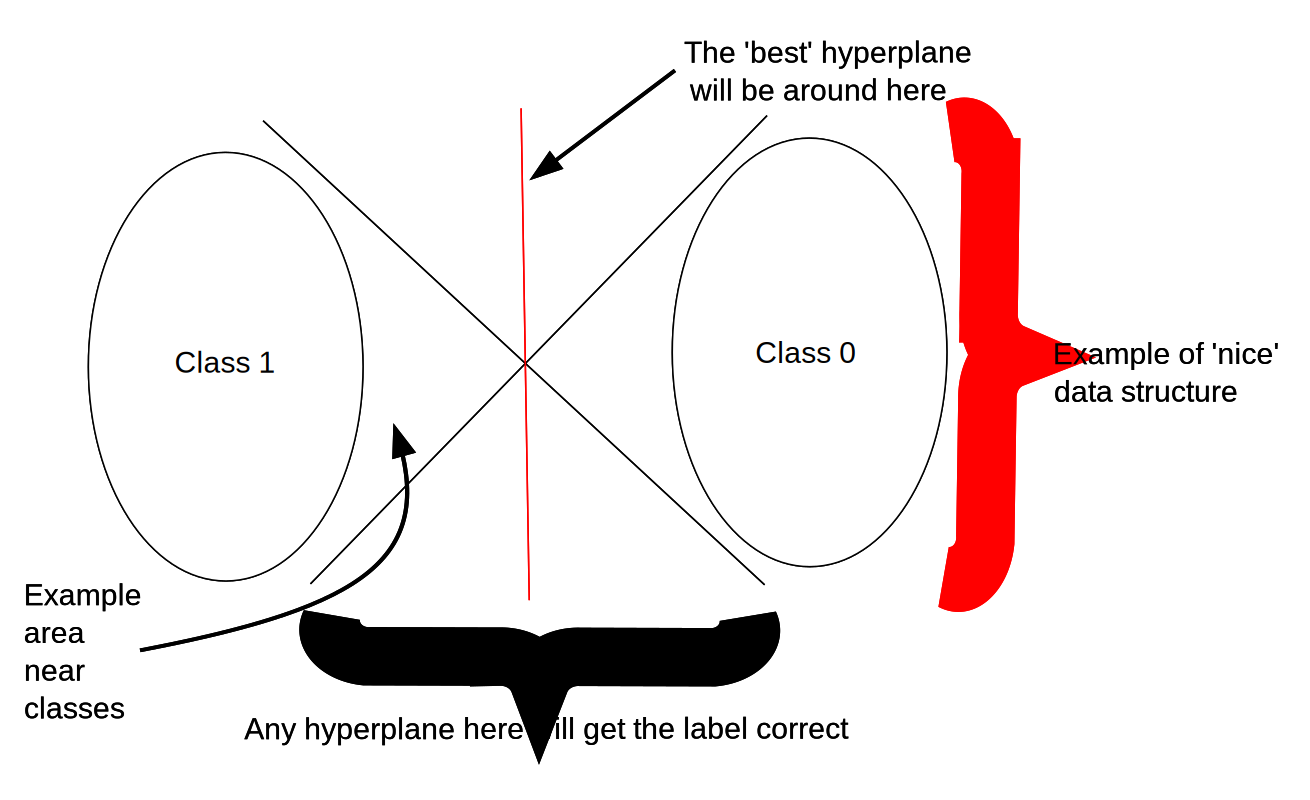
\includegraphics[width=\textwidth]{figs/hyperplanes_good_classes.png}}
\caption{Illustration of well separated classes.} 
\label{fig:good_sep_classes} % labels must come after captions (figures are 'labelable'?)
\end{figure}

Figure \ref{fig:good_sep_classes} shows the desired geometry of the data. In the following two scenarios our reasoning makes the assumption when new examples are fed into the algorithm. They will likely be somewhere around the classes. The ovals indicate the 'clouds' of data that define each class and each line indicates a \gls{decisionboundary}. In a 2D context, this is a line and in a n-d context, these would be \gls{hyperplane}s.  For illustrative purposes, this is a 2D scenario, but it is important to recognise this would generalise up to n-many dimensions.  In this instance, 

\begin{figure}[H]
    \centering
    \makebox[\textwidth]{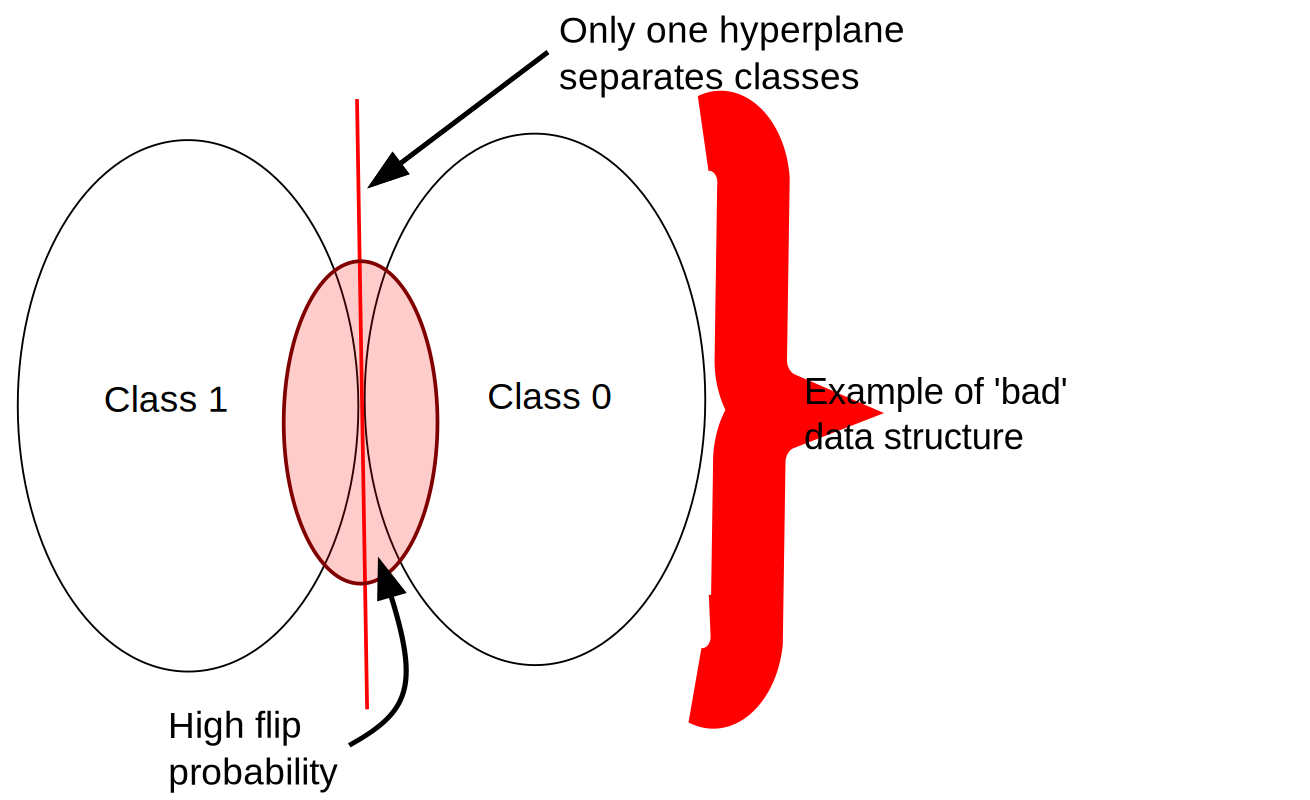
\includegraphics[width=\textwidth]{figs/hyperplanes_poor_classes.png}}
    \caption{Illustration of poorly separated classes.}{With classes that have data grouped close together geometrically, we see there is a smaller range of separating hyperplanes that can be found (in this strictly hypothetically instance, there is only one meaningfully distinct hyperplane) and if we draw new samples from these classes, we might expect the data generating process to generate examples that are misclassified (and so experience a label 'flip') by the trained classifier.}
    \label{fig:poor_sep_classes}
\end{figure}

Figure \ref{fig:poor_sep_classes} shows a geometry of the data that would have high flipping probability upon \gls{rp}. There is only one \gls{hyperplane} that separates the classes. Hence new examples (e.g. out-of-sample data), which are likely to be near this boundary (the area indicated in red) have a high chance of being misclassified. This is an example of a situation where a traditional loss function, such as the \gls{mse}, would have poor \gls{generalisationperformance}, upon learning a \gls{decisionboundary} between these two classes. \bigskip

Calculation of empirical \gls{fp} (compressing the data via \gls{rp}s) allows for a proxy of how separable the classes are. However, any single \gls{rp} is not likely to find a good representation of the data. We define a 'good representation' as a representation that allows for accurate and rapidly learning on the data, compared to attempting to learn on a 'raw' transformed version of the data.

% the above paragraph fails to mention the disconnect between gradient based learning and using flip probability - you need to mention this somewhere

Hence, we wish to find a good representation of the data, through many repeated  \gls{rp}s, that shifts the classes away from each other geometrically (i.e. from Figure \ref{fig:poor_sep_classes} to Figure \ref{fig:good_sep_classes}) and hence minimises the \gls{fp} \bigskip

For this, we will need an empirical measure of \gls{fp} and a functioning (trainable) implementation of it in a \gls{cnn}. \bigskip

\gls{fp}
\chapter{Methods}

One of the motivations of using flip probability as a loss function is the 'cold start' problem in \gls{ml}. Ideally, one could 'warm start' a network by training it from scratch with a small sample. This is not dissimilar to the idea of \gls{dataaugmentation} - improving the ability of the network to learn on the raw data. This is a problem that is exacerbated further in the context of \gls{dl}, as there are many more millions of parameters (in modern networks) and hence the \gls{parameterspace} is much larger. One hypothesis is that one could use \gls{fp} to perform \gls{representationlearning} on less data than would usually be required so that the network will train quickly.

\begin{hypothesis} %\begin{hyp}[H\ref{hyp:first}] \label{hyp:first}
Using \gls{fp} to perform \gls{representationlearning} on the data will allow the network to train more quickly.
\label{hyp:first}
\end{hypothesis}

% this is something of a false dichotomy - need to investigate how CE performs around edges
Another problem with classifiers trained using a traditional loss function, like \gls{mse}, is that (as illustrated by figures \ref{fig:poor_sep_classes} and \ref{fig:good_sep_classes}) they tend to generalise poorly, especially when the data classes are closely spaced geometrically. Hence, by using \gls{fp} to find a representation of the data that spaces out these classes in a geometric sense, we might expect to see an increase in \gls{generalisationperformance}.

\begin{hypothesis} %\begin{hyp}[H\ref{hyp:first}] \label{hyp:first}
Using \gls{fp} to perform \gls{representationlearning} on the data will improve \gls{generalisationperformance}.
\label{hyp:second}
\end{hypothesis}

Another key idea, as mention in 

\section{Flip Probability}

We have some data:

\begin{equation}
X \in \mathds{R}^d 
\end{equation}

Where $d$, the dimensionality of the data, is quite high. \bigskip

For a single batch of data and a single classifier, the flipping probability can be thought of as the proportion of label 'flips' that occur when the classifier and data are randomly projected down (using a \gls{rp} matrix) to a lower dimension:

\begin{equation}
P((R h)^T Rx \neq h^{T}x)  
\end{equation}

An example of a (linear) classifier is a single neuron in a \gls{nn} at the last layer. Randomly projecting the classifier and minimising the \gls{fp} can act as a proxy for learning a classifier on the projected space. \smallskip

 \gls{fp} can then be defined empirically:

\begin{equation}
\hat{P}\ := \\ P(\frac{1}{m}\sum_{j = 1}^m (R_j h)^T R_{j}x \neq h_i^{T}x)  
\end{equation}

Where;  \smallskip

\begin{itemize}
\item $\hat{P}$ is the empirical estimate of the flipping probability  
\item $R$ is the \gls{rp} matrix  
\item $P$ is the proportion of inequalities recorded over the data 
\item $h_i$ is the classifier  
\end{itemize}

If  \gls{fp} is small, the points are well separated. \bigskip

The entries of $R$ are typically drawn from a normal distribution (and will be in this instance) but can also be drawn from other distributions in order to speed up generation of the random (projection) matrices while training the network:

\begin{equation}
R \in M^{kxd}, R_{ij} \stackrel{i.i.d}{\backsim} N(0,1) 
\end{equation}

When $d$ is very large, subgaussian random variables can be used replacements. One such alternative is the Rademacher discrete distribution:

\begin{equation}
R \in M^{kxd}, R_{ij} = \pm 1 \; w.p. 0.5 
\end{equation}

\begin{itemize}
\item $M$ is the number of classes  
\item $k$ is the projection dimension, a user specified parameter 
\item $R_{ij}$ is an individual entry of the \gls{rp} matrix  \gls{sgd}  
\end{itemize}

One example of $h_i$ is the ZAMBINGO at the $i^{th}$ node of the last layer of an \gls{mlp}. This would take the form of a vector of weights that are applied to (cross-multiplied with) the inputs from the previous layer and a bias term is added, before the \gls{activationfunction} for the layer is added.
\bigskip

\bigskip

\gls{fp} implemented using  \gls{sgd} would look like the following:

\begin{equation}
\label{eq:sgd_fp}
\hat{P}\ := \frac{1}{L}\frac{1}{M}\sum_{l = 1}^N \sum_{j = 1}^M \mathds{1}((R_j h_i)^T R_jx_L \neq h_i^Tx_L)  
\end{equation}

Where;  \smallskip

\begin{itemize}
\item $\mathds{1}$ is the \gls{indicatorfunction}  
\item $k$ is the projection dimension, a user specified parameter 
\item $R_{ij}$ is an individual entry of the \gls{rp} matrix  \gls{sgd} 
\item $x_L$ is the batch of data used during  \gls{sgd}  
\item $N$ is the number of batches of data used in  \gls{sgd}  
\item $M$ is the number of classes %is the number of \gls{rp} matrices
\end{itemize}

Equation \ref{eq:sgd_fp} fails to consider the possibility that the randomly projected classifier,  $(R_j h_i)$, will classify the data, $x_L$, correctly where the unprojected classifier has classified the data incorrectly.
\bigskip

\begin{equation}
\label{eq:conditional_sgd_fp}
\hat{P}\ := \frac{1}{L}\frac{1}{M}\sum_{l = 1}^N \sum_{j = 1}^M  \mathds{1}( (R_j h_i)^T R_jx_L \neq h_i^Tx_L \mid \hat{h_i^T}x_L = y_i )  
\end{equation}

Where $y_i$ is the correct label of the data $x_i$. 
\bigskip

Equation \ref{eq:conditional_sgd_fp} correctly accounts for this (although it is anticipated with a well trained classifier, this situation would account for a negligible proportion of cases). 
\bigskip

How often the projected classifier incorrectly classifies the data when the data is compressed strongly depends on the  geometry of the data. The key idea with using  \gls{fp} as a loss function in a  \gls{nn} context is to "drive the representation to a nice place" aka, undergo effective unsupervised representation learning before learning a classifier on the data. 
\bigskip

% TODO - more explain on FP

Implementing  \gls{fp} inevitably encounters a problem in that loss functions must be differentiable, if the network is to be trained using gradient descent, or a variant thereof (such as the \gls{adam} algorithm). In particular, the loss function must be differentiable with respect to the parameters of the model in order for the gradients to be backpropagated through the network. The gradients are then used to update the parameters in the correct direction (towards a local, and hopefully global, optimum). Modern tools incorporate auto-differentiation libraries to lessen the mathematical challenge of specifying derivatives for complex loss functions, but the function, when decomposed, must still nonetheless be differentiable.
\bigskip

Hence, a major challenge with the above loss functions is that they are not differentiable, primary due to the inequality involved. This inequality introduces a discontinuity in the function, which is not differentiable. One way to get around this is to recognise that in principle, we are minimising the angle between the 

\section{Implementation of Flip Probability}

One way we can reduce the computational burden of this procedure is to generate the \gls{rp} matrices at the start of the algorithm instead of dynamically each time the loss function is called. This has the disadvantage of introducing dependencies \cite{bob_rp_storage}, but given the number of \gls{rp} matrices needed to be generated in even a small \gls{cnn}, this is a necessary step in order for testing and iteration to be feasible. 
\bigskip

% TODO - calculate number of RP matrices need for static storage and dynamic generation
\section{Data sets}
 
\subsection{Artificial Data}

In order to test the effectiveness of \gls{fp} as a loss function, some synthetic, linearly separable data was generated. As  \gls{fp} benefits from the  \gls{jll}, it was necessary to ensure this was sufficiently highly dimensional. Hence, data with dimension $k =$ 5,10,20,50,100,500,1000,10000 was generated to test with a  \gls{nn}. 
\bigskip

 \subsection{MNIST}
 
\gls{mnist} is a famous data set often regarded as a starting point to work on and experiment with. It represents an improvement over the older \gls{nist} data set, which used images from different sources (high school students and workers) for the training and testing set \cite{nist}. It comprises of images of handwritten digits (of ten classes, 0-9), scaled, centered and batch normalised into 28x28 grayscale images. Of 60k images, these are split into 10k training images and 50k testing images \cite{mnist}. This type of problem (digit recognition) is fairly unique in image classification in that the visual information directly conveys the \gls{classlabel}, i.e. there is a direct mapping between the image and the label. Modern training accuracies are sufficiently high (less than 0.2\%, \cite{mnist_sota}) on \gls{mnist} that it can be considered a 'solved' problem \cite{mnist_sota_web}. However, this data is of sufficiently dimensionality ($\mathds{R}^{784}$) that it can adequately be used as a test for \gls{fp} in a \gls{cnn} context. 
 \bigskip

\subsection{CIFAR-10}

To extend upon the \gls{mnist} testing with a more challenging data set, the ten class \gls{cifar}-10 data set was used. Here, the mapping between image and label is less direct, and the complexity of the images (which include animal and vehicles) is increased.
\bigskip

Tiny ImageNet:

Tiny ImageNet is smaller version of the well-known \gls{ilsvrc} ImageNet, which has over a million images.

\section{Testing Schemes}
  
First, it is necessary to have baseline results. While there are various data preprocessing (scaling, whitening,  and data augmentation strategies (e.g. flipping, cropping, rotation and jittering)  available, we use a fairly simple script in Pytorch (\cite{mnist_script}) that uses the test/train split present in the  \gls{mnist} data set and rapidly achieves an accuracy of 97\%. Ideally, we would test the algorithms using 10 fold- \gls{cv} (the 'gold standard', \ref{algo:10-fold-cv}). However, this introduces a high level of computational burden, as the algorithm must be run independently across at least 10 subsets of the data. 
\bigskip

% ZAMBINGO - cv algorithm
\begin{algorithm}[H]
\SetAlgoLined
\KwResult{Write here the result }
 initialization\;
 \While{While condition}{
  instructions\;
  \eIf{condition}{
   instructions1\;
   instructions2\;
   }{
   instructions3\;
  }
 }
    \caption{The 10 fold \gls{cv} algorithm}
    \label{algo:10-fold-cv}
\end{algorithm}

\bigskip

Instead, for a reasonable test of \gls{generalisationperformance}, we can use the typical test-train split, where 10\% of the data is used for testing and 90\% is used for training. This split is randomly determined.
\bigskip

In terms of \gls{hyperparameter} tuning, various modern methods for this exist, the simplest of which is the grid search. This also results in a high computational burden, being a brute force strategy. 

\begin{wrapfigure}{l}{0.5\textwidth}
    \includegraphics[scale=0.5]{figs/relu.png}
    \caption{The ReLu activation function.}
    \label{fig:relu_function}
\end{wrapfigure}

The \gls{relu} (figure \ref{fig:relu_function}) was used as the activation function in all testing schemes. This is an \gls{activationfunction} that is fast to compute, easy to interpret, widely used, and performs well in neural networks generally (\cite{activation_search}). 
\bigskip

% Zambingo - formatting is borked here
In all cases;

\begin{itemize}
    \item Batch size = 64
    \item The optimisation method was \gls{sgd}
    \item The learning rate was 0.01
\end{itemize}

\begin{landscape}

%\newgeometry{left=0.5cm,top=0.5cm,bottom=0.5cm,right=0.5cm}

\begin{table}[hp]
    \centering
    \begin{tabular}{ |p{1cm}||p{2cm}|p{1cm}|p{1cm}|p{1cm}|p{1cm}|p{1cm}|p{6cm}| }
         \hline
         \multicolumn{8}{|c|}{Scheme Parameters} \\
         \hline
         No. & Epochs & $M$ & Loss & 2nd Loss & DO & $N$ & Notes\\
         \hline
         1 & 100 & - &FP &CE &0.5 &Y & Alt. Loss per batch\\
         2 & 10 & - &FP &CE &0.5 &Y & Alt. Loss per batch\\
         3 & 10 & - &FP &CE & - &Y & Alt. Loss per batch\\
         4 & 10 & - &FP &CE & - &Y & Alt. Loss per batch\\
         5 & 5 & -  &FP &CE & - &Y & Alt. Loss per batch\\
         6 & 10 & -  &FP &CE & - &Y & Alt. Loss over run\\
         7 & 5 & 0.5 &FP &CE & - &Y & Alt. Loss over run\\
         8 & 10 & 0.5 &FP &CE & - &Y & Alt. Loss over run\\
         9 & 10 & 0.5 &FP &CE &0.5 &Y & Short FP periods, alternating\\
         10 & 10 & 0.5 &CE & - &0.5 &Y & Baseline\\
         11 & 10 & 0.5 &CE & - & - &N &Baseline - No Normalisation\\
         12 & 20 & - &FP &CE & - &Y & Switched loss at midpoint*\\
         13 & 100 & - &FP &CE & -  &Y & Switched loss at midpoint*\\
         \hline
         \multicolumn{3}{@{}p{1.5in}}{\footnotesize (DO) $=$ Drop-out}\\
         \multicolumn{3}{@{}p{1.5in}}{\footnotesize ($M$) $=$ Momentum}\\
         \multicolumn{3}{@{}p{1.5in}}{\footnotesize ($N$) $=$ Normalisation}\\
         \multicolumn{3}{@{}p{1.5in}}{\footnotesize (-) $=$ Unused}\\
         \multicolumn{3}{@{}p{1.5in}}{\footnotesize (*) $=$ Keeping layers frozen as appropriate} 
    \end{tabular}
    \caption{Testing Schemes run on MNIST}
    \label{table:testing_schemes}
\end{table}

\end{landscape}

%\restoregeometry

\section{Hardware}

When benchmarking for running time, the \gls{nn}s were run on an Asus laptop with 8 \gls{gb}s of \gls{ram}, a Intel Core i5-8250U processor and a 256\gls{gb} \gls{ssd}. All operations were run on the \gls{cpu}. \href{https://colab.research.google.com/}{Google colaboratory}, a cloud notebook platform, was also used to run networks.
\chapter{Results and Discussion}

The first set of experiments used the 'toy' artificial data set. \bigskip

The second set of experiments used the MNIST data set. In principle, any modern iteration of a \gls{cnn} can achieve very high accuracy on this data set \cite{sota_web}. \gls{nn}s ranging from simple CNNs to modern CapsNets, \gls{resnet}s and DenseNets (all \gls{dnn}s) should be able to achieve 98-99\% on this data set {\cite{mnist_sota_web}}. This is seen in the test and training accuracies in the baseline training schemes (figure \ref{fig:training_scheme_10_11}), where very high accuracies are achieved after only a few \gls{epoch}s. 
\bigskip

% https://tex.stackexchange.com/questions/140833/arranging-multiple-plots-in-a-grid-inside-a-figure-subfloat

\begin{figure}[H]
    \centering
    \subfloat[first]{
      \includegraphics[width=65mm]{figs/run_1/test_accuracy_fp.png}
    }
    \subfloat[second]{
      \includegraphics[width=65mm]{figs/run_1/test_losses_fp.png}
    }
    \hspace{0mm}
    \subfloat[third]{
      \includegraphics[width=65mm]{figs/run_1/train_accuracy.png}
    }
    \subfloat[forth]{
      \includegraphics[width=65mm]{figs/run_1/train_losses_ce.png}
    }
    \hspace{0mm}
    \hbox to 67.5mm{}% !!
    \subfloat[fifth]{   % ???
      \includegraphics[width=65mm]{figs/run_1/train_losses_fp.png}
    }
    \caption{The results of the initial training scheme}
    \label{fig:training_scheme_1}
    \end{figure}
    
    \begin{figure}
    \centering
    \subfloat[first]{
      \includegraphics[width=65mm]{figs/run_2/test_accuracy_fp.png}
    }
    \subfloat[second]{
      \includegraphics[width=65mm]{figs/run_2/test_losses_fp.png}
    }
    \hspace{0mm}
    \subfloat[third]{
      \includegraphics[width=65mm]{figs/run_2/train_accuracy.png}
    }
    \subfloat[forth]{
      \includegraphics[width=65mm]{figs/run_2/train_losses_ce.png}
    }
    \hspace{0mm}
    \hbox to 67.5mm{}% !!
    \subfloat[fifth]{   % ???
      \includegraphics[width=65mm]{figs/run_2/train_losses_fp.png}
    }
    \caption{The results of the second training scheme}
    \label{fig:training_scheme_2}

\end{figure}

\begin{figure}[H]
    \centering
    \subfloat[first]{
      \includegraphics[width=65mm]{figs/run_3/test_accuracy_fp.png}
    }
    \subfloat[second]{
      \includegraphics[width=65mm]{figs/run_3/test_losses_fp.png}
    }
    \hspace{0mm}
    \subfloat[third]{
      \includegraphics[width=65mm]{figs/run_3/train_accuracy.png}
    }
    \subfloat[forth]{
      \includegraphics[width=65mm]{figs/run_3/train_losses_ce.png}
    }
    \hspace{0mm}
    \hbox to 67.5mm{}% !!
    \subfloat[fifth]{   % ???
      \includegraphics[width=65mm]{figs/run_3/train_losses_fp.png}
    }
    \caption{The results of the third training scheme}
    \label{fig:training_scheme_3}
\end{figure}

\begin{figure}[H]
    \centering
    \subfloat[first]{
      \includegraphics[width=65mm]{figs/run_4/test_accuracy_fp.png}
    }
    \subfloat[second]{
      \includegraphics[width=65mm]{figs/run_4/test_losses_fp.png}
    }
    \hspace{0mm}
    \subfloat[third]{
      \includegraphics[width=65mm]{figs/run_4/train_accuracy.png}
    }
    \subfloat[forth]{
      \includegraphics[width=65mm]{figs/run_4/train_losses_ce.png}
    }
    \hspace{0mm}
    \hbox to 67.5mm{}% !!
    \subfloat[fifth]{   % ???
      \includegraphics[width=65mm]{figs/run_4/train_losses_fp.png}
    }
    \caption{The results of the fourth training scheme}
    \label{fig:training_scheme_4}
\end{figure}

\begin{figure}[H]
    \centering
    \subfloat[first]{
      \includegraphics[width=65mm]{figs/run_5/test_accuracy_fp.png}
    }
    \subfloat[second]{
      \includegraphics[width=65mm]{figs/run_5/test_losses_fp.png}
    }
    \hspace{0mm}
    \subfloat[third]{
      \includegraphics[width=65mm]{figs/run_5/train_accuracy.png}
    }
    \subfloat[forth]{
      \includegraphics[width=65mm]{figs/run_5/train_losses_ce.png}
    }
    \hspace{0mm}
    \hbox to 67.5mm{}% !!
    \subfloat[fifth]{   % ???
      \includegraphics[width=65mm]{figs/run_5/train_losses_fp.png}
    }
    \caption{The results of the fifth training scheme}
    \label{fig:training_scheme_5}
\end{figure}

\begin{figure}[H]
    \centering
    \subfloat[first]{
      \includegraphics[width=65mm]{figs/run_6/test_accuracy_fp.png}
    }
    \subfloat[second]{
      \includegraphics[width=65mm]{figs/run_6/test_losses_fp.png}
    }
    \hspace{0mm}
    \subfloat[third]{
      \includegraphics[width=65mm]{figs/run_6/train_accuracy.png}
    }
    \subfloat[forth]{
      \includegraphics[width=65mm]{figs/run_6/train_losses_ce.png}
    }
    \hspace{0mm}
    \hbox to 67.5mm{}% !!
    \subfloat[fifth]{   % ???
      \includegraphics[width=65mm]{figs/run_6/train_losses_fp.png}
    }
    \caption{The results of the sixth training scheme}
    \label{fig:training_scheme_6}
\end{figure}

\begin{figure}[H]
    \centering
    \subfloat[first]{
      \includegraphics[width=65mm]{figs/run_7/test_accuracy_fp.png}
    }
    \subfloat[second]{
      \includegraphics[width=65mm]{figs/run_7/test_losses_fp.png}
    }
    \hspace{0mm}
    \subfloat[third]{
      \includegraphics[width=65mm]{figs/run_7/train_accuracy.png}
    }
    \subfloat[forth]{
      \includegraphics[width=65mm]{figs/run_7/train_losses_ce.png}
    }
    \hspace{0mm}
    \hbox to 67.5mm{}% !!
    \subfloat[fifth]{   % ???
      \includegraphics[width=65mm]{figs/run_7/train_losses_fp.png}
    }
    \caption{The results of the seventh training scheme}
    \label{fig:training_scheme_7}
\end{figure}

\begin{figure}[H]
    \centering
    \subfloat[first]{
      \includegraphics[width=65mm]{figs/run_8/test_accuracy_fp.png}
    }
    \subfloat[second]{
      \includegraphics[width=65mm]{figs/run_8/test_losses_fp.png}
    }
    \hspace{0mm}
    \subfloat[third]{
      \includegraphics[width=65mm]{figs/run_8/train_accuracy.png}
    }
    \subfloat[forth]{
      \includegraphics[width=65mm]{figs/run_8/train_losses_ce.png}
    }
    \hspace{0mm}
    \hbox to 67.5mm{}% !!
    \subfloat[fifth]{   % ???
      \includegraphics[width=65mm]{figs/run_8/train_losses_fp.png}
    }
    \caption{The results of the eighth training scheme}
    \label{fig:training_scheme_8}
\end{figure}

\begin{figure}[H]
    \centering
    \subfloat[first]{
      \includegraphics[width=65mm]{figs/run_9/test_accuracy_fp.png}
    }
    \subfloat[second]{
      \includegraphics[width=65mm]{figs/run_9/test_losses_fp.png}
    }
    \hspace{0mm}
    \subfloat[third]{
      \includegraphics[width=65mm]{figs/run_9/train_accuracy.png}
    }
    \subfloat[forth]{
      \includegraphics[width=65mm]{figs/run_9/train_losses_ce.png}
    }
    \hspace{0mm}
    \hbox to 67.5mm{}% !!
    \subfloat[fifth]{   % ???
      \includegraphics[width=65mm]{figs/run_9/train_losses_fp.png}
    }
    \caption{The results of the ninth training scheme}
    \label{fig:training_scheme_9}
\end{figure}

\begin{figure}[H]
    \centering
    \subfloat[normalised]{
      \includegraphics[width=65mm]{figs/run_10/test_accuracy_fp.png}
    }
    \subfloat[normalised]{
      \includegraphics[width=65mm]{figs/run_10/test_losses_fp.png}
    }
    \hspace{0mm}
    \subfloat[normalised]{
      \includegraphics[width=65mm]{figs/run_10/train_accuracy.png}
    }
    \subfloat[normalised]{
      \includegraphics[width=65mm]{figs/run_10/train_losses_ce.png}
    }
    \hspace{0mm}
    \subfloat[no normalisation]{
      \includegraphics[width=65mm]{figs/run_11/test_accuracy_fp.png}
    }
    \subfloat[no normalisation]{
      \includegraphics[width=65mm]{figs/run_11/test_losses_fp.png}
    }
    \hspace{0mm}
    \subfloat[no normalisation]{
      \includegraphics[width=65mm]{figs/run_11/train_accuracy.png}
    }
    \subfloat[no normalisation]{
      \includegraphics[width=65mm]{figs/run_11/train_losses_ce.png}
    }
    \hspace{0mm}
    
    \caption{The results of the tenth and eleventh training scheme, the baseline scheme, with and without normalisation}
    \label{fig:training_scheme_10_11}
\end{figure}

%\begin{figure}
%\centering
%
%
%\caption{The results of the eleventh training scheme, the baseline with no normalisation}
%\label{fig:training_scheme_11}
%\end{figure}

\begin{figure}[H]
    \centering
    \subfloat[first]{
      \includegraphics[width=65mm]{figs/run_12/test_accuracy_fp.png}
    }
    \subfloat[second]{
      \includegraphics[width=65mm]{figs/run_12/test_losses_fp.png}
    }
    \hspace{0mm}
    \subfloat[third]{
      \includegraphics[width=65mm]{figs/run_12/train_accuracy.png}
    }
    \subfloat[forth]{
      \includegraphics[width=65mm]{figs/run_12/train_losses_ce.png}
    }
    \hspace{0mm}
    \hbox to 67.5mm{}% !!
    \subfloat[fifth]{   % ???
      \includegraphics[width=65mm]{figs/run_12/train_losses_fp.png}
    }
    \caption{The results of the twelfth training scheme}
    \label{fig:training_scheme_12}
\end{figure}

\begin{figure}[H]
    \centering
    \subfloat[first]{
      \includegraphics[width=65mm]{figs/run_13/test_accuracy_fp.png}
    }
    \subfloat[second]{
      \includegraphics[width=65mm]{figs/run_13/test_losses_fp.png}
    }
    \hspace{0mm}
    \subfloat[third]{
      \includegraphics[width=65mm]{figs/run_13/train_accuracy.png}
    }
    \subfloat[forth]{
      \includegraphics[width=65mm]{figs/run_13/train_losses_ce.png}
    }
    \hspace{0mm}
    \hbox to 67.5mm{}% !!
    \subfloat[fifth]{   % ???
      \includegraphics[width=65mm]{figs/run_13/train_losses_fp.png}
    }
    \caption{The results of the thirteenth training scheme}
    \label{fig:training_scheme_13}
\end{figure}

We can see that the baseline schemes, 10/11, clearly achieve a very high accuracy rapidly and without trouble. Removing image normalisation slightly decreases training and testing accuracy during the early stages of training, but otherwise has little effect on the final accuracy.

The third, more refined set of experiments was on the \gls{cifar}-10 data set

The final experiment was an attempt to implement \gls{fp} in a \gls{dl} context, to see if any improvements could be made. We used the Tiny ImageNet data set

\section{Discussion}

Other work leveraging \gls{rp}s exists. For example, \gls{rp}s have been used in projection networks in tandem with the full \gls{nn} to efficiently compress down (reduce the number of parameters) the full networks to lessen the memory footprint. This allows projection networks to run on devices that have resource constraints, such as smartwatches \cite{projection_net}. 



\include{tex/conclusion}
\chapter{Appendix}

\printglossary[type=\acronymtype]
\printglossary[type=main]

\pagebreak

\chapter{Appendix}

\printglossary[type=\acronymtype]
\printglossary[type=main]

\pagebreak

%Sets the bibliography style to UNSRT and imports the 
%bibliography file "dissertation.bib".
\bibliographystyle{unsrt}
\bibliography{dissertation}

\end{document} 

